% ================================================================
%  第 1 章 七则数学俳句 (Seven mathematical haikus)
%  依据原书 PDF 第 1--19 页译出；编号审计见文件末尾注释
% ================================================================

\chapter{七则数学俳句}

\epigraph{月光之下, \\紫藤的花色与芬芳, \\仿佛都很遥远。}{与谢芜村（Yosa Buson）}

在数学中, 我们常常要付出艰苦的努力才能证明定理；而即便运气好, 遇到的也往往是复杂的证明, 它们也要求可能的读者付出大量的劳动. 为一条出色的数学陈述找到一个聪明而简短的证明, 是难得的成功. 让我们把缪斯的这些珍贵馈赠称为\newterm{mathematical-haiku}{数学俳句}{mathematical haiku}——大多数数学家肯定都珍藏了好几个例子. 下面是我偏爱的几个.

\section{凸集上 Fritz John 引理的一个几何证明}

\begin{theorem}\label{thm:1.1}
设 $K \subset \R^n$ 是内部非空的紧凸集, $E$ 是包含 $K$ 的体积最小的\newterm{ellipsoid}{椭球}{ellipsoid}. 则有包含关系
$\frac{1}{n}E \subset K$
（其中 $\frac{1}{n}E$ 表示由 $E$ 关于其中心以比率 $1/n$ 收缩得到的椭球）.
\end{theorem}

一个有趣的例子是顶点为 $(P_0, P_1, \ldots, P_n)$（其中向量 $P_1 - P_0, \ldots, P_n - P_0$ 线性无关）的 $(n+1)$-单形 $\sum(P_0, P_1, \ldots, P_n)$:
\begin{align*}
  \sum(P_{0},P_{1},\ldots,P_{n})
  =\Big\{P\in\R^{n}\Big|P=\sum_{j=0}^{n} t_{j} P_{j},
  \text{ 其中 } 0\leq t_{0},t_{1},\ldots,t_{n}\leq 1,\ \sum_{j=0}^{n} t_{j}=1\Big\}.
\end{align*}
当 $\dist(P_{j}, P_{k})$ 对所有不同的顶点对都相同时, 称该单形为\newterm{equilateral-simplex}{等边单形}{equilateral simplex}.

在 $\R^n$ 中内接于某个球面的所有 $(n+1)$-单形中, 体积最大者必为等边单形——一个直接的几何论证即可证明这一点. 由此可得: 给定任一 $(n+1)$-单形 $T$, 存在唯一的包含 $T$ 的体积最小椭球 $E$: 这个 $E$ 是把内接于等边 $(n+1)$-单形 $T'$ 的外接球面, 经把 $T'$ 映为 $T$ 的仿射变换所得到的象.

这一事实有一个对偶的说法: 在包含给定等边 $(n+1)$-单形的所有椭球中, 体积最小者是其外接球面.

\begin{proof}
首先注意, 包含 $K$ 的体积最小椭球的存在性由紧性论证容易得到；而且, 如等边 $(n+1)$-单形的情形所示, 收缩因子 $1/n$ 是精确的.

我们用反证法. 假设存在紧\newterm{convex-set}{凸集}{convex set} $K$, 使得 $\frac{1}{n}E$ 不包含于 $K$. 由于仿射变换保持紧的、有界的凸集类以及椭球类, 不失一般性可设 $E$ 是一个球. 取一点 $P \in (\frac{1}{n}E) \cap (\R^n - K)$, 用 $H$ 表示过 $P$ 且不与 $K$ 相交的一张超平面, 即 $K$ 包含在 $H$ 所界定的两个半空间之一（记为 $H^+$）中（见图~\ref{fig:1.1}, 其中 $K$ 包含在 $E$ 的虚线部分之内）.

\begin{figure}[htbp]
\centering
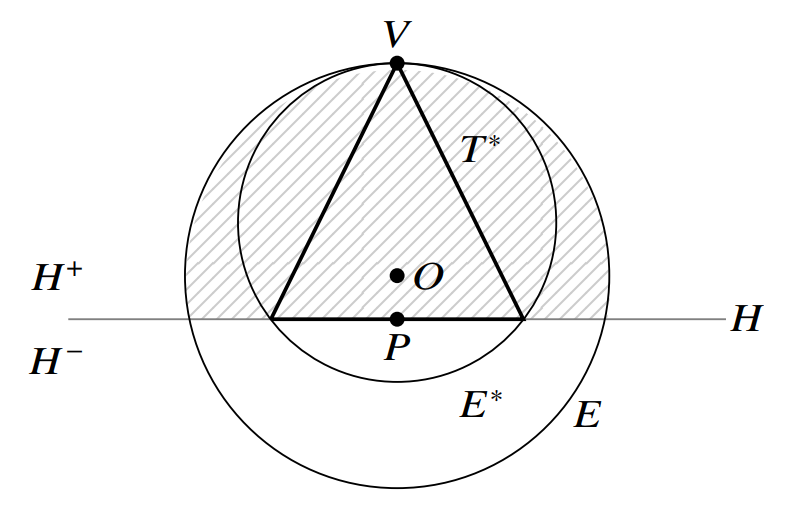
\includegraphics[width=0.5\textwidth]{figs/fig-1-1.png}
\caption{Fritz John 引理.}
\label{fig:1.1}
\end{figure}

作一个等边 $(n+1)$-单形 $T^*$, 使其一个顶点位于 $V$（放在虚线区域 $E \cap H^+$ 的边界与 $E$ 的过 $P$ 的直径的交点处）, 而其余 $n$ 个顶点位于超平面 $H$ 内以 $P$ 为心的 $(n-1)$-球面 $S^*$ 上: $S^* = H \cap E^*$, 其中 $E^*$ 是 $T^*$ 的外接球. 设 $A$ 是保持直线 $OP$ 不动且把 $S^*$ 映为 $S = E \cap H$ 的仿射变换. 那么 $A(E^*)$ 是包含 $A(T^*)$ 的体积最小椭球. 特别地, 有严格不等式 $\vol(E) > \vol(A(E^*))$. 但 $A(E^*) \supseteq E \cap H^+ \supseteq K$, 这与 $E$ 作为包含 $K$ 的体积最小椭球的选取相矛盾.
\end{proof}

Fritz John 给出的\thmref{thm:1.1}的原始证明 \cite{b35} 是不同的, 而且复杂得多. 这条引理在多个理论中扮演重要角色. 例如, 它是把与凸集相联系的极大函数化归为对平行多面体取平均这一特殊情形的恰当工具. 大约 1969 年, 当我还是本科生、在 M.~de Guzmán 的实变函数课上学习时, 应老师之请, 我与同学 A.~Gallego 合作, 为这条有趣的引理寻找一个初等的几何证明. 我们的证明在 1970 年冬于（西班牙）穆尔西亚召开的西班牙数学会会议上作为短篇报告宣读, 后来收录在 \cite{b29,b32} 中. 我相信如今它只被视为凸分析中的一个民间结果, 它曾被多人使用, 其中包括 L.~Caffarelli 在其关于 Monge--Ampère 方程的工作 \cite{b21} 中, 以及 C.~Fefferman 在其 Whitney 扩张结果 \cite{b33} 中.

\section{$\zeta(2)$ 的一个初等计算}

著名的恒等式 $\sum_{n=1}^{\infty}1/n^2 = \pi^2/6$ 最初由 L.~Euler 利用 $\sin(z)/z$ 的无穷乘积展开证明, 但它也可以作为贝塞尔恒等式应用于函数 $y = x$（$0 < x < 1$）的傅里叶系数的推论得到. 如今文献中还可以找到若干别的证明, 它们把 $\zeta(2)$ 的计算化归为适当平面区域上的二重积分；下面我们给出其中一种的细节.

\begin{theorem}\label{thm:1.2}
我们有
\begin{align*}
  \sum_{n=1}^{\infty}\frac{1}{n^{2}}=\frac{\pi^{2}}{6}.
\end{align*}
\end{theorem}

\begin{proof}
写
\begin{align*}
  \zeta(2)=\sum_{n=1}^{\infty}\frac{1}{(2n)^{2}}+\sum_{n=0}^{\infty}\frac{1}{(2n+1)^{2}}.
\end{align*}
即
\begin{align*}
  \zeta(2)
  &=\frac{4}{3}\sum_{n=0}^{\infty}\frac{1}{(2n+1)^{2}}
   =\frac{1}{3}\sum_{n=0}^{\infty}\Big(\int_{-1}^{+1}x^{2n}\,\mathrm{d}x\Big)^{2}
   =\frac{1}{3}\sum_{n=0}^{\infty}\int_{-1}^{+1}\int_{-1}^{+1}(x^{2}y^{2})^{n}\,\mathrm{d}x\,\mathrm{d}y\\
  &=\frac{1}{3}\int_{-1}^{+1}\int_{-1}^{+1}\frac{\mathrm{d}x\,\mathrm{d}y}{1-x^{2}y^{2}}.
\end{align*}
变量替换
\begin{align*}
  x=\tanh(s)=\frac{\exp(s)-\exp(-s)}{\exp(s)+\exp(-s)}, \qquad
  y=\tanh(t)=\frac{\exp(t)-\exp(-t)}{\exp(t)+\exp(-t)}, \qquad
  -\infty<s,\,t<+\infty,
\end{align*}
给出
\begin{align*}
  \zeta(2)=\frac{1}{3}\int_{-\infty}^{\infty}\int_{-\infty}^{\infty}
  \frac{\mathrm{d}s\,\mathrm{d}t}{\cosh(s)^{2}\cosh(t)^{2}-\sinh(s)^{2}\sinh(t)^{2}}.
\end{align*}
但由于双曲函数
\begin{align*}
  \cosh(s)=\frac{\exp(s)+\exp(-s)}{2}, \qquad
  \sinh(s)=\frac{\exp(s)-\exp(-s)}{2}
\end{align*}
满足恒等式
\begin{align*}
  \cosh(s)\cosh(t)-\sinh(s)\sinh(t)=\cosh(s-t),
\end{align*}
\begin{align*}
  \cosh(s)\cosh(t)+\sinh(s)\sinh(t)=\cosh(s+t),
\end{align*}
我们得到
\begin{align*}
  \zeta(2)=\frac{1}{3}\int_{-\infty}^{\infty}\int_{-\infty}^{\infty}
  \frac{\mathrm{d}s\,\mathrm{d}t}{\cosh(s-t)\cosh(s+t)}.
\end{align*}
再作变量替换 $u = s - t$, $v = s + t$, 得
\begin{align*}
  \zeta(2)=\frac{1}{6}\int_{-\infty}^{\infty}\int_{-\infty}^{\infty}
  \frac{\mathrm{d}u\,\mathrm{d}v}{\cosh(u)\cosh(v)}
  =\frac{2}{3}\Big(\int_{0}^{\infty}\frac{\mathrm{d}z}{1+z^{2}}\Big)^{2}
  =\frac{\pi^{2}}{6},
\end{align*}
其中用到了替换 $x = \log z$, $z > 0$.
\end{proof}

\begin{remark}\label{rem:1.3}
如前所述, 这条著名公式有许多不同的证明. Euler 的原始证明的优点是还能给出 $\zeta$ 在一切正偶数 $2k$ 处的值, 但这里给出的证明位居最直接、最简单者之列. 与双曲正切相联系的变量替换的想法是一次奇妙的意外收获: 当时我正在写一篇关于 Ginzburg--Landau 模型中相变的文章, 同时又应西班牙数学会期刊 La Gaceta de la Real Sociedad Matemática Española 的编辑之邀, 撰写一篇综述文章 \cite{b26}, 介绍我对 R.~Apéry 的 $\zeta(3)$ 无理性证明的 1979 年未刊版本. 于是, 在计算 $\zeta(2)$ 与 $\zeta(3)$ 的同时, 图象 $y = \tanh(x/\varepsilon)$ 正作为 $+1$ 与 $-1$ 两态之间相变的例子出现在我的另一项工作中.
\end{remark}

\section{$\zeta(3)$ 的无理性}

公式
\begin{align*}
  \zeta(3)=\sum_{n=1}^{\infty}\frac{1}{n^{3}}
  =-\frac{1}{2}\int_{0}^{1}\int_{0}^{1}\frac{\log(st)}{1-st}\,\mathrm{d}s\,\mathrm{d}t
\end{align*}
由熟知的恒等式
\begin{align*}
  \int_{0}^{1}\int_{0}^{1}\frac{s^{\alpha+\gamma}t^{\alpha+\gamma}}{1-st}\,\mathrm{d}s\,\mathrm{d}t
  =\sum_{n=1}^{\infty}\frac{1}{(\alpha+\gamma+n)^{2}}
\end{align*}
对 $\gamma$ 求导并在 $\gamma = 0$ 处取值得到:
\begin{align*}
  \int_{0}^{1}\int_{0}^{1}\frac{s^{\alpha}t^{\alpha}\log(st)}{1-st}\,\mathrm{d}s\,\mathrm{d}t
  =-2\sum_{n=1}^{\infty}\frac{1}{(\alpha+n)^{3}}.
\end{align*}
因此, 若 $\alpha$ 是非负整数, 则得
\begin{align*}
  \int_{0}^{1}\int_{0}^{1}\frac{s^{\alpha}t^{\alpha}\log(st)}{1-st}\,\mathrm{d}s\,\mathrm{d}t
  =-2\Big\{\zeta(3)-\sum_{n=1}^{\alpha}\frac{1}{n^{3}}\Big\},\quad\text{若 } \alpha\geq 1,
\end{align*}
以及
\begin{align*}
  \int_{0}^{1}\int_{0}^{1}\frac{\log(st)}{1-st}\,\mathrm{d}s\,\mathrm{d}t
  =-2\zeta(3),\quad\text{若 } \alpha= 0.
\end{align*}
类似地, 若整数 $\alpha > \beta$, 则有
\begin{align*}
  \int_{0}^{1}\int_{0}^{1}\frac{s^{\alpha+\gamma}t^{\beta+\gamma}}{1-s t}\,\mathrm{d}s\,\mathrm{d}t
  =\frac{1}{\alpha-\beta}\sum_{n=1}^{\infty}
  \left\{\frac{1}{n+\beta+\gamma}-\frac{1}{n+\alpha+\gamma}\right\},
\end{align*}
对 $\gamma$ 求导并在 $\gamma = 0$ 处取值, 得
\begin{align*}
  \int_{0}^{1}\int_{0}^{1}\frac{s^{\alpha}t^{\beta}\log(st)}{1-st}\,\mathrm{d}s\,\mathrm{d}t
  =-\frac{1}{\alpha-\beta}\sum_{n=\beta+1}^{\alpha}\frac{1}{n^{2}}.
\end{align*}
因此, 若 $Q(s,t)$ 是整系数多项式, 且对每个变量分别为 $n$ 次, 则有
\begin{align*}
  \int_{0}^{1}\int_{0}^{1}\frac{Q(s,t)\log(s t)}{1-s t}\,\mathrm{d}s\,\mathrm{d}t
  =A_{n}\zeta(3)+B_{n},
\end{align*}
其中 $A_{n}$ 是整数, $B_{n}$ 是有理数, 其分母整除 $d_{n}^{3}$, 这里
\begin{align*}
  d_{n}=\operatorname{lcm}(1,2,\ldots,n).
\end{align*}
为证明 $\zeta(3)$ 的\newterm{irrationality}{无理性}{irrationality}, 目标是找一列多项式 $P_n(s, t)$, 它对每个变量的次数都 $\leq n$, 且使积分
\begin{align*}
  \int_{0}^{1}\int_{0}^{1}\frac{P_{n}(s,t)\log(s\cdot t)}{1-s t}\,\mathrm{d}s\,\mathrm{d}t
\end{align*}
非零但非常小. 结果表明, 一个好的选择是
\begin{align*}
  P_{n}(s,t)=P_{n}(s)P_{n}(t),
\end{align*}
其中
\begin{align*}
  P_{n}(s)=\frac{1}{n!}\left(\frac{d}{ds}\right)^{n}[s^{n}(1-s)^{n}]
\end{align*}
是 Legendre 多项式.

为计算
\begin{align*}
  \int_{0}^{1}\int_{0}^{1}\frac{P_{n}(s)P_{n}(t)\log(s t)}{1-s t}\,\mathrm{d}s\,\mathrm{d}t,
\end{align*}
使用公式
\begin{align*}
  \frac{\log(st)}{1-st}=\int_{0}^{1}\frac{\mathrm{d}u}{1-(1-st)u}
\end{align*}
是方便的. 我们得到
\begin{align*}
  \int_{0}^{1}\int_{0}^{1}\frac{P_{n}(s)P_{n}(t)\log(st)}{1-st}\,\mathrm{d}s\,\mathrm{d}t
  &=\int_{0}^{1}\int_{0}^{1}\int_{0}^{1}\frac{P_{n}(s)P_{n}(t)}{1-(1-st)u}\,\mathrm{d}s\,\mathrm{d}t\,\mathrm{d}u\\
  &=\int_{0}^{1}\int_{0}^{1}\int_{0}^{1}
   \frac{s^{n}t^{n}\cdot u^{n}(1-s)^{n}P_{n}(t)}{[1-(1-st)u]^{n+1}}\,\mathrm{d}s\,\mathrm{d}t\,\mathrm{d}u,
\end{align*}
这里对 $s$ 变量做了分部积分. 然后变量替换
\begin{align*}
  u=\frac{1-v}{1-(1-s t)v},\qquad
  \mathrm{d}u=\frac{-s t}{[1-(1-s t)v]^{2}}\,\mathrm{d}v
\end{align*}
给出
\begin{align*}
  \int_{0}^{1}\int_{0}^{1}\int_{0}^{1}
  \frac{(1-s)^{n}(1-v)^{n}P_{n}(t)}{1-(1-st)v}\,\mathrm{d}s\,\mathrm{d}t\,\mathrm{d}v,
\end{align*}
再对 $t$ 分部积分一次, 得
\begin{align*}
  0&<\int_{0}^{1}\int_{0}^{1}\frac{P_{n}(s)P_{n}(t)\log(st)}{1-st}\,\mathrm{d}s\,\mathrm{d}t\\
  &=\int_{0}^{1}\int_{0}^{1}\int_{0}^{1}
   \frac{s^{n}(1-s)^{n}\, t^{n}(1-t)^{n}\, v^{n}(1-v)^{n}}{[1-(1-st)v]^{n+1}}\,\mathrm{d}s\,\mathrm{d}t\,\mathrm{d}v\\
  &\leq C\Big[\max_{0\leq s,t,v\leq 1}
   \frac{s(1-s)t(1-t)v(1-v)}{1-(1-st)v}\Big]^{n}
   =C\left(\sqrt{2}-1\right)^{4n}.
\end{align*}
但
\begin{align*}
  d_{n}=\operatorname{lcm}(1,2,\cdots,n)
  =\prod_{\substack{p\,\text{素数}\\ p\leq n}}p^{\left\lbrack\log n/\log p\right\rbrack}
  \leq\prod_{p\leq n}p^{\log n/\log p}=n^{\pi(n)}
  \leq n^{(1+\varepsilon)n/\log n}=e^{n(1+\varepsilon)}
\end{align*}
对每个 $\varepsilon > 0$ 成立, 其中用素数定理估计了
\begin{align*}
  \pi(n)=\operatorname{card}\left\{p\ \text{素数}\leq n\right\}.
\end{align*}

\begin{theorem}\label{thm:1.4}
$\zeta(3)$ 是无理数.
\end{theorem}

\begin{proof}
由于 $(\sqrt{2}-1)^4 e^3 < 1$, 上面的构造给出一列用有理数 $E_n/D_n$ 对 $\zeta(3)$ 的逼近, 使得
\begin{align*}
  0<\Big|\zeta(3)-\frac{E_{n}}{D_{n}}\Big|=o\Big(\frac{1}{D_{n}}\Big).
\end{align*}
\end{proof}

$\zeta(3)$ 无理性的第一个证明由 R.~Apéry \cite{b18} 得到, 并在 1978 年于赫尔辛基召开的国际数学家大会上报告. 上面的证明受 C.~L.~Siegel 工作的启发, 那年秋天我在普林斯顿高等研究院由 E.~Bombieri 与 B.~Dwork 组织并主持的讨论班上学到了它.

Siegel \cite{b39} 考虑了下面的问题:

求两个 $n$ 次整系数多项式 $A(x)$ 与 $B(x)$, 使差 $e^x - A(x)/B(x)$ 在 $0$ 处有 $n + 1$ 阶零点.

这一条件意味着
\begin{align*}
  B(x)e^{x}-A(x)=R(x)=cx^{2n+1}+\cdots,
\end{align*}
其中 $R(x)$ 是以 $2n+1$ 阶项开头的幂级数.

用待定系数写出 $A$ 与 $B$, 并让 $0, \ldots, 2n$ 阶项相等, 就得到关于 $A$ 与 $B$ 的 $2n+2$ 个系数的 $2n+1$ 个齐次线性方程. 这表明方程组有系数 $c \neq 0$ 的非平凡解. 逐次求导, 得到
\begin{align*}
  D^{n+1}R=D^{n+1}(Be^{x})=e^{x}(1+D)^{n+1}B=c_{0}x^{n}+\cdots,
\end{align*}
其中 $c_{0} = (2n + 1)\cdot(2n)\cdots(n + 1)\,c$. 于是
\begin{align*}
  (1+D)^{n+1}B=e^{-x}\left(c_{0}x^{n}+\cdots\right),
\end{align*}
又因 $B$ 是 $n$ 次多项式, 得
\begin{align*}
  (1+D)^{n+1}B=c_{0}x^{n}.
\end{align*}
类似地,
\begin{align*}
  (-1+D)^{n+1}A=c_{0}x^{n},
\end{align*}
我们可以自由选取 $c$ 使 $c_{0}=1$. 即
\begin{align*}
  B=\left(1+D\right)^{-n-1}x^{n},\qquad
  A=\left(-1+D\right)^{-n-1}x^{n},\qquad
  D^{n+1}R=x^{n}e^{x}.
\end{align*}
接下来考虑
\begin{align*}
  J^{k+1}\phi(x)=\int_{0}^{x}\frac{(x-t)^{k}}{k!}\phi(t)\,\mathrm{d}t.
\end{align*}
注意
\begin{align*}
  D^{k}J^{k}\phi=\phi,\qquad J^{k}D^{k}\phi=\phi,
\end{align*}
只要 $\phi(0) = D\phi(0) = \cdots = D^{k-1}\phi(0)$. 还要注意
\begin{align*}
  D^{k}(e^{\lambda x}\phi)=e^{\lambda x}(\lambda+D)^{k}\phi.
\end{align*}
这些公式给出了算子 $(\pm1+D)^{-k}$, 并证明了: 若 $Q$ 是整系数多项式, 则 $(\pm1+D)^{-k}Q$ 也是整系数的. 特别地,
\begin{align*}
  R(x)=\frac{x^{n+1}}{n!}\int_{0}^{1}(1-t)^{n}t^{n}e^{x t}\,\mathrm{d}t
  =\frac{x^{2n+1}}{n!}\int_{0}^{1}P_{n}(t)e^{x t}\,\mathrm{d}t,
\end{align*}
其中
\begin{align*}
  P_{n}(x)=\frac{1}{n!}\frac{d^{n}}{\mathrm{d}x^{n}}\{x^{n}(1-x)^{n}\}
\end{align*}
是 $n$ 阶 Legendre 多项式.

Siegel 观察到
\begin{align*}
  0<|R(x)|\leq\frac{|x|^{2n+1}}{n!}e^{|x|},
\end{align*}
由此推出
\begin{align*}
  0<|B_{n}(m)e^{m}-A_{n}(m)|\leq\frac{m^{2n+1}e^{m}}{n!},
\end{align*}
$e$ 的任何整数幂 $e^m$ 的无理性由此容易得到. 这些估计启发了上述 Apéry 定理的证明.

有几个月, 我一直试图把方法推广到 $\zeta(2m+1)$ 的其他值而没有成功；随后我得知, F.~Beukers 已独立地投寄了一篇稿件 \cite{b19}, 其证明非常相似甚至几乎相同, 于是我决定不发表我的证明——尽管当时我已在威斯康星大学（麦迪逊）与普林斯顿大学作过关于它的公开报告. 不过, 这一方法仍有余地去估计不同的 $\zeta(2m+1)$ 的许多有理系数线性组合. 这项工作由 T.~Rivoal \cite{b38} 完成, 他证明了由 $1, \zeta(3), \ldots, \zeta(2m+1)$ 在有理数域上张成的向量空间的维数 $\geq \frac{1}{2}\log(m)$. 特别地, 这蕴含序列 $\{\zeta(2m+1)\}$ 包含无穷多个无理数.

\section{拉普拉斯算子分数幂的一个逐点不等式}

傅里叶变换
\begin{align*}
  \widehat{f}(\xi)=\int_{\mathbb{R}^{n}}e^{-i x\cdot\xi}f(x)\,\mathrm{d}x,
\end{align*}
作用于 $\R^n$ 上的\newterm{laplacian}{拉普拉斯算子}{Laplacian} $\Delta u = \sum_{i=1}^{n} u_{x_i x_i}$, 对速降光滑函数 $u$ 给出表示
\begin{align*}
  \widehat{\Delta u}(\xi)=-|\xi|^{2}\widehat{u}(\xi).
\end{align*}
于是可以由公式
\begin{align*}
  \widehat{\Lambda^{\alpha}u}(\xi)=|\xi|^{\alpha}\widehat{u}(\xi)
\end{align*}
定义 $-\Delta$ 的\newterm{fractionary-powers}{分数幂}{fractionary powers}. 当 $0 < \alpha < 2$ 时, 有表示
\begin{align*}
  \Lambda^{\alpha}u(x)=C_{\alpha,n}\int_{\mathbb{R}^{n}}\frac{u(x)-u(y)}{|x-y|^{n+\alpha}}\,\mathrm{d}y,
\end{align*}
其中
\begin{align*}
  C_{\alpha,n}=2^{\alpha-2}\bigl(\alpha^{2}+\alpha(n-2)\bigr)
  \Gamma\Big(\frac{n-2+\alpha}{2}\Big)\Gamma\Big(1-\frac{\alpha}{2}\Big)>0,
\end{align*}
由此清楚地看到算子 $\Lambda^{\alpha}$ 的非局部特征. 然而, 对 $C^1$ 凸函数 $\phi$, 下列逐点不等式成立.

\begin{theorem}\label{thm:1.5}
设 $\phi$ 是 $C^{1}$ 凸函数. 则
\begin{align*}
  \Lambda^{\alpha}(\phi(f))(x)\leq\phi^{\prime}(f)(x)\cdot\Lambda^{\alpha}f(x).
\end{align*}
\end{theorem}

\begin{proof}
我们有
\begin{align*}
  \Lambda^{\alpha}(\phi(f))(x)
  &=C_{\alpha,n}\int_{\mathbb{R}^{n}}\frac{\phi(f)(x)-\phi(f)(y)}{|x-y|^{n+\alpha}}\,\mathrm{d}y\\
  &\leq C_{\alpha,n}\int_{\mathbb{R}^{n}}\frac{\phi^{\prime}(f)(x)(f(x)-f(y))}{|x-y|^{n+\alpha}}\,\mathrm{d}y
  =\phi^{\prime}(f)(x)\,\Lambda^{\alpha}f(x).
\end{align*}
\end{proof}

尽管证明简单 \cite{b27,b30}, 鉴于所涉算子 $\Lambda^{\alpha}$ 的非局部性, 其有效性仍令人惊讶. 它对非线性与非局部的发展问题也有若干有趣的应用. 下面简述其一.

水波的分析, 或多孔介质中的 Muskat 流与 Hele--Shaw 流, 都涉及两种流体之间、或流体与真空之间自由界面的演化. 在两种情形中, 都有一条曲线（在 $\R^2$ 中）或一张曲面（在 $\R^3$ 中）, 其时间演化须由基本定律（水波的 Bernoulli 定律、多孔介质的 D'Arcy 定律）控制, 并且可以给运动边界指定一个速度场, 从而得到一个由相当复杂的非线性微分方程组成的封闭系统 \cite{b28}.

然而, 人们很早就发现, 在如此的一般性下问题是不适定的. 在多孔介质的情形, Rayleigh 首先、其后 Taylor 观察到, 当某个量 $\sigma$ 变为负时, 线性化问题是不稳定的. 因此, 为建立相容的理论, 还需要在假设 $\sigma$ 于时刻 $t = 0$ 为正的前提下控制 $\sigma$ 的演化. 选取自由边界的适当（等温）参数化 $\psi: \R \to \R^2$（或 $\psi: \R^2 \to \R^3$）, 就导致对 Sobolev 范数的演化的估计: $\frac{d}{dt} \|\Lambda^\alpha \psi\|_T^2$.

经过一些代数操作, 任务化归为下述情形:
\begin{align*}
  \frac{d}{d t}\left\|\Lambda^{\alpha}\psi\right\|_{L^{2}}^{2}
  \leq-\sum_{j}\sum_{|\alpha|=k}\int\sigma(x,t)D_{x}^{\alpha}\psi(x,t)\,\Lambda D_{x}^{\alpha}\psi(x,t)\,\mathrm{d}x
  +O\big(\left\|\Lambda^{k}\psi\right\|_{L^{2}}^{p}\big),
\end{align*}
其中 $p > 0$.

于是, 我们不等式的特殊情形
\begin{align*}
  u(x)\,\Lambda u(x)\geq\frac{1}{2}\Lambda u^{2}(x)
\end{align*}
连同 Rayleigh--Taylor 项 $\sigma$ 的正性, 使我们能够处理上式中的危险项并得出适定性.

\section{广义拉普拉斯算子与极小曲面}

设 $f$ 是定义在欧氏空间 $\R^n$ 的开区域上的局部可积函数. 其广义拉普拉斯算子 $\Delta^\star f$ 由下述极限（若它存在）给出:
\begin{align*}
  \Delta^{\star}f(x):=\lim_{r\rightarrow0^{+}}\frac{2(n+2)}{r^{2}}\fint_{B_{r}^{(n)}(x)}(f(y)-f(x))\,\mathrm{d}y.
\end{align*}
这里记号 $\fint_{B_r^{(n)}(x)}$ 表示在以 $x$ 为心、半径 $r$ 的球 $B_r^{(n)}(x) \subset \R^n$ 上的平均, $\mathrm{d}y = \mathrm{d}\mu_n(y)$ 是 $\R^n$ 上的 Lebesgue 测度, 而 $\mu_n(A) = |A| = \mathrm{vol}(A)$ 是可测集 $A$ 的测度.

众所周知, 连续的广义调和函数（即对每个 $x$ 都有 $\Delta^\star f(x) = 0$）必是光滑的, 从而按通常意义调和: $\Delta f = 0$.

然而, 存在广义意义下调和的不连续函数. 一个例子是
\begin{align*}
  f(x^{\prime},x_{n})=
  \begin{cases}
    \alpha_{+}, & \text{若 } x_{n}>0,\\
    \frac{1}{2}\left(\alpha_{+}+\alpha_{-}\right), & \text{若 } x_{n}=0,\\
    \alpha_{-}, & \text{若 } x_{n}<0,
  \end{cases}
\end{align*}
其中 $x = (x', x_n)$ 表示欧氏空间 $\R^n$（$n \geq 2$）中的点；当 $\alpha_+ \neq \alpha_-$ 时它显然不连续, 却处处满足 $\Delta^\star f(x) = 0$.

设 $S$ 是把区域 $\Omega$ 分成两个非空部分的光滑曲面:
\begin{align*}
  \Omega=\Omega^{+}\cup\Omega^{-}\cup S,\qquad
  S=\partial\Omega^{+}\cap\Omega=\partial\Omega^{-}\cap\Omega.
\end{align*}
令函数 $f_S$ 在 $\Omega^+$ 内等于 $\alpha_+$, 在 $\Omega^-$ 内等于 $\alpha_-$, 在 $S$ 上等于 $\frac{1}{2}(\alpha_++\alpha_-)$.

\begin{theorem}\label{thm:1.6}
函数 $f_S$（设 $\alpha_+ \neq \alpha_-$）为广义调和, 当且仅当 $S$ 是\newterm{minimal-surface}{极小曲面}{minimal surface}.
\end{theorem}

在证明中, 我们将使用一致椭圆方程粘性解的现代概念. 也就是说, 我们将证明: 若 $\Delta^\star f_S = 0$, 则局部地 $S$ 是极小曲面方程的一个粘性解的图象, 因而它必是光滑的. 我们还将用到极小曲面与椭圆方程的若干熟知性质；\cite{b22} 与 \cite{b34} 是合适的参考文献.

\section*{一个基本的微积分引理}

设 $S$ 是 $\R^n$ 中的光滑（$C^4$）超曲面, 带单位法向量场 $\nu(x)$. 给定 $x \in S$ 与足够小的 $r > 0$, 球 $B_r^{(n)}(x)$ 被 $S$ 分成两个连通分支 $S_r^+(x)$ 与 $S_r^-(x)$, 其中 $S_r^+(x)$（相应地, $S_r^-(x)$）由 $B_r^{(n)}(x)$ 中沿给定法方向位于 $S$ 之上（相应地, 之下）的点组成.

则有下列结论.

\begin{lemma}\label{lem:1.7}
当 $r \to 0^+$ 时,
\begin{align*}
  \mathrm{vol}(S_{r}^{+}(x))-\mathrm{vol}(S_{r}^{-}(x))
  =-c_{n} H_{S}(x)\cdot r^{n+1}+O(r^{n+3}),
\end{align*}
其中 $H_{S}(x)$ 表示 $S$ 在点 $x$ 处的\newterm{mean-curvature}{平均曲率}{mean curvature}, $c_{n} > 0$ 是仅依赖于维数 $n$ 的普适常数.
\end{lemma}

\begin{proof}
不失一般性, 可设 $x = 0$ 是一个坐标系的原点, 且 $S$ 在 $x$ 处的切空间是水平的, 即法向量 $\nu(0) = (0, \ldots, 0, 1)$. 于是在 $x = 0$ 附近, $S$ 是光滑（$C^4$）函数 $x_n = \varphi(x_1, \ldots, x_{n-1})$ 的图象, 满足
\begin{align*}
  \varphi(0)=0,\qquad \nabla\varphi(0)=0.
\end{align*}
于是, 在圆柱 $B_r^{(n-1)}(0) \times \R$ 内部, 对足够小的 $r$, 有包含关系
\begin{align*}
  S\cap(B_{r}^{(n-1)}(0)\times\R)\subset\{x\in\R^{n}:|x_{n}|\leq c_{1}r^{2}\},
\end{align*}
其中正常数 $c_{1}$ 依赖于 $\varphi$ 的二阶导数的大小.

一个初等的计算表明, $S \cap B_r^{(n)}(0)$ 到 $B_r^{(n-1)}(0)$ 的竖直投影必包含球
\begin{align*}
  B_{r-c_{2}r^{3}}^{(n-1)}(0),
\end{align*}
其中 $c_{2}$ 是固定常数. 令
\begin{align*}
  D_{r}^{+}=B_{r}^{(n)}(0)\cap\Omega^{+}\cap\{|x_{n}|\leq c_{1}r^{2}\},\qquad
  D_{r}^{-}=B_{r}^{(n)}(0)\cap\Omega^{-}\cap\{|x_{n}|\leq c_{1}r^{2}\}.
\end{align*}
则因 $S$ 含于该带形区域内, 由对称性得第一个等式
\begin{align*}
  \mathrm{vol}(S_{r}^{+}(0))-\mathrm{vol}(S_{r}^{-}(0))
  &=\mathrm{vol}(D_{r}^{+})-\mathrm{vol}(D_{r}^{-})\\
  &=\int_{B_{r-c_{2}r^{3}}^{(n-1)}(0)}(c_{1}r^{2}-\varphi(x))\,\mathrm{d}x
   -\int_{B_{r-c_{2}r^{3}}^{(n-1)}(0)}(c_{1}r^{2}+\varphi(x))\,\mathrm{d}x+I,
\end{align*}
其中 $I$ 是积分区域受限所致的修正项.

直接计算 $I$ 项可得
\begin{align*}
  |I|\lesssim r^{2}\cdot\bigl(r^{n-1}-(r-c_{2}r^{3})^{n-1}\bigr)\lesssim r^{n+3}=O\bigl(r^{n+3}\bigr).
\end{align*}
因此
\begin{align*}
  \mathrm{vol}(S_{r}^{+}(0))-\mathrm{vol}(S_{r}^{-}(0))
  =-2\int_{B_{r-c_{2}r^{3}}^{(n-1)}(0)}\varphi(x)\,\mathrm{d}x+O(r^{n+3}).
\end{align*}
再对圆柱体积作一次估计, 给出
\begin{align*}
  \bigg|\int_{B_{r}^{(n-1)}(0)}\varphi(x)\,\mathrm{d}x-\int_{B_{r-c_{2}r^{3}}^{(n-1)}(0)}\varphi(x)\,\mathrm{d}x\bigg|
  \lesssim r^{n+3}=O(r^{n+3}).
\end{align*}
然后 Taylor 展开给出
\begin{align*}
  \int_{B_{r}^{(n-1)}(0)}\varphi(y)\,\mathrm{d}y
  =\frac{1}{2(n+1)}\,\Delta\varphi(0)\cdot r^{2}+O(r^{4}).
\end{align*}
至此可以完成引理的证明, 因为已知
\begin{align*}
  H_{S}(x^{\prime},\varphi(x^{\prime}))
  =\frac{1}{n-1}\operatorname{div}\Big(\frac{\nabla\varphi}{\sqrt{1+|\nabla\varphi|^{2}}}\Big)(x^{\prime}),
\end{align*}
且由 $\nabla\varphi(0)=0$ 有
\begin{align*}
  H_{S}(0)=\frac{1}{n-1}\Delta\varphi(0).
\end{align*}
\end{proof}

\section*{证明的完成}

首先, 不失一般性, 可以设 $\alpha_+ = +1$ 且 $\alpha_- = -1$. 其次注意到, 定理的两个蕴涵关系之一是直接的: 若 $S$ 极小且 $C^1$, 则由 de Giorgi--Nash 的经典定理, $S$ 必光滑, 从而可以应用\lemref{lem:1.7}, 对任意点 $x \in S$ 有
\begin{align*}
  \Delta^{\star}f(x)
  &=\lim_{r\to0^{+}}\frac{2(n+2)}{r^{2}}\fint_{B_{r}^{(n)}(x)}(f(y)-0)\,\mathrm{d}y\\
  &=\lim_{r\to0^{+}}\frac{2(n+2)}{|B_{r}^{(n)}(x)|\,r^{2}}
   [\mathrm{vol}(S_{r}^{+}(x))-\mathrm{vol}(S_{r}^{-}(x))]=0,
\end{align*}
这由极小性条件 $H_{S}(x)=0$ 得到.

注意, 用\lemref{lem:1.7} 作类似论证也可以证明: $f_S$ 广义调和蕴含 $S$ 极小. 因此, 为完成证明, 只须证明 $S$ 的 $C^4$ 正则性.

为继续证明, 回忆: 定义在 $\Omega \times \R \times \R^n \times M^n$ 上的实连续函数 $F$（其中 $M^n$ 表示 $n \times n$ 对称矩阵组成的向量空间）给出一个椭圆方程 $F(x, u, Du, D^2u) = 0$, 若
\begin{align*}
  F(x,u,\eta,\delta)\leq F(x,u,\eta,\delta+\sigma)
\end{align*}
对一切 $(x, u, \eta, \delta) \in \Omega \times \R \times \R^n \times M^n$ 及非负的 $\sigma \in M^n$ 成立.

若存在正常数 $\lambda$ 与 $\Lambda$ 满足估计
\begin{align*}
  0<\lambda\left\|\sigma\right\|<F(x,u,\eta,\delta+\sigma)-F(x,u,\eta,\delta)\leq\Lambda\left\|\sigma\right\|,
\end{align*}
则称该椭圆方程是一致椭圆的, 其中 $\|\sigma\|$ 表示 $(L^2, L^2)$-范数（即 $\|\sigma\| = \sup_{\|x\|=1} \|\sigma x\|$, 亦即 $\sigma$ 的最大特征值）.

\begin{definition}\label{def:1.8}
设 $u$ 是连续函数. 若对任意二次多项式 $\Psi \in C^2(\Omega)$ 以及 $u - \Psi$ 的局部极大（相应地, 局部极小）值点 $x_0$, 都有
\begin{align*}
  F(x_{0},u(x_{0}),D\Psi(x_{0}),D^{2}\Psi(x_{0}))\geq 0\quad(\text{相应地},\ \leq 0),
\end{align*}
则称 $u$ 为 $F(x,u,Du,D^2u) = 0$ 的粘性下解（相应地, 粘性上解）.

最后, 若 $u$ 既是粘性下解又是粘性上解, 则称之为粘性解.
\end{definition}

文献 \cite{b22} 含有关于一致椭圆方程粘性解的正则性（见其 Corollary 5.7）与唯一性（见其 Corollary 5.4）的结果, 我们将引用它们来结束证明.

更精确地说, 在假设
\begin{align*}
  \Delta^{\star}f\equiv 0
\end{align*}
之下, 设 $P$ 是在点 $x = (x_1, \ldots, x_{n-1}, x_n) \in S \cap P$ 处从下方与我们的超曲面 $S = \{x_n = \varphi(x_1, \ldots, x_{n-1})\}$ 相切的抛物面.

设 $f_{P}$ 是引言中对它定义的相应函数. 我们有不等式
\begin{align*}
  \fint_{B_{r}^{(n)}(x)}f_{P}\,\mathrm{d}x\geq\fint_{B_{r}^{(n)}(x)}f_{S}\,\mathrm{d}x.
\end{align*}
另一方面, 对超曲面 $P$ 应用\lemref{lem:1.7} 给出
\begin{align*}
  \int_{B_{r}^{(n)}(x)}f_{P}\,\mathrm{d}x=-c_{n}H_{P}(x)\cdot r^{n+1}+O(r^{n+2}),
\end{align*}
它与假设
\begin{align*}
  \lim_{r\to0^{+}}\frac{1}{r^{2}}\fint_{B_{r}^{(n)}(x)}f_{S}\,\mathrm{d}y=0
\end{align*}
一起, 蕴含
\begin{align*}
  H_{P}(x)\leq 0.
\end{align*}
类似地, 若 $P$ 现是在点 $x$ 处从上方与 $S$ 相切的抛物面, 则必有 $H_P(x) \geq 0$. 因此, $\varphi$ 是方程
\begin{align*}
  \operatorname{div}\left(\frac{\nabla\varphi}{\sqrt{1+|\nabla\varphi|^{2}}}\right)=0
\end{align*}
的粘性解, 其一致椭圆性由 $S$ 属于 $C^{1}$ 类这一假设保证.

此类解的正则性理论 \cite{b34} 使我们可以断定 $\varphi$（以及 $S$）的光滑性, 从而其极小性.

\section{弧上的格点}

函数
\begin{align*}
  r(n)=\#\{n=a^{2}+b^{2}:a,b\in\Z\},
\end{align*}
它计数整数 $n$ 表为两平方和的表法个数, 是数论中的一个重要角色.

利用 $n$ 的素因子分解可以得到一个著名的公式. 设
\begin{align*}
  n=2^{\nu}\prod_{\substack{p_{j}\equiv 1\;(\mathrm{mod}\;4)}}p_{j}^{\alpha_{j}}
  \prod_{\substack{q_{k}\equiv 3\;(\mathrm{mod}\;4)}}q_{k}^{\beta_{k}}.
\end{align*}
则有
\begin{enumerate}
\item[(i)] 若某个 $\beta_k$ 为奇数, 则 $r(n) = 0$；
\item[(ii)] 若对每个 $k$, $\beta_k = 2\beta'_k$ 都是偶数, 则 $r(n) = 4 \prod_j (1 + \alpha_j)$,
\end{enumerate}
由此推出
\begin{equation}\label{eq:1.1}
  \limsup_{n\to\infty}\frac{r(n)}{(\log n)^{p}}=\infty,\quad\text{对每个 } p>0,
\end{equation}
\begin{equation}\label{eq:1.2}
  \limsup_{n\to\infty}\frac{r(n)}{n^\varepsilon}=0,\quad\text{对每个 } \varepsilon>0.
\end{equation}
既然 $r(n)$ 表示以原点为心、半径 $R = \sqrt{n}$ 的圆上的\newterm{lattice-point}{格点}{lattice point} $(a,b) \in \Z^2$ 的个数, 那么 \eqref{eq:1.1} 表明: 对某些足够大的 $R$, 在这种圆上可以找到我们所希望的任意多的格点.

另一方面, 若 $\nu_j = (a_j, b_j)$, $j = 1, 2, 3$, 是半径 $R = \sqrt{n}$ 的圆上的三个格点, 则归功于亚历山大的 Hero 的著名定理给出恒等式
\begin{align*}
  \left\|\nu_{1}-\nu_{2}\right\|\left\|\nu_{2}-\nu_{3}\right\|\left\|\nu_{3}-\nu_{1}\right\|=4\Delta\cdot R,
\end{align*}
其中 $\Delta$ 是以 $\{\nu_1, \nu_2, \nu_3\}$ 为顶点的三角形的面积, 它至少是 $1/2$. 因此, 含这三点 $\nu_1, \nu_2, \nu_3$ 的\newterm{arc}{弧}{arc} $C$ 必满足
\begin{align*}
  \mathrm{length}(C)\geq(2R)^{1/3}.
\end{align*}

\begin{theorem}\label{thm:1.9}
对每个 $1/3 \leq \alpha < 1/2$, 存在有限常数 $C_\alpha$, 使得在以原点为心、半径 $R$ 的圆上, 任何长度为 $R^\alpha$ 的弧至多包含 $C_\alpha$ 个格点（对 $R$ 一致）.
\end{theorem}

\begin{proof}
(a) 众所周知, $r(n)$ 的性质在高斯整数环中才能得到最好的揭示. 对奇素数 $p \equiv 1 \pmod{4}$, 除明显的对称性 $p = (\pm a)^2 + (\pm b)^2 = (\pm b)^2 + (\pm a)^2$ 外, 表示是唯一的, 我们约定选取
\begin{align*}
  a+b\,\mathrm{i}=\sqrt{p}\;e^{2\pi i\Phi},\quad 0<b<a,\quad
  0<\Phi=\frac{1}{2\pi}\arctan\frac{b}{a}<\frac{1}{4}.
\end{align*}
若
\begin{align*}
  n=2^{\nu}\prod_{p_{j}\equiv 1\,(\mathrm{mod}\,4)}p_{j}^{\alpha_{j}}
  \prod_{q_{k}\equiv 3\,(\mathrm{mod}\,4)}q_{k}^{2\beta_{k}},
\end{align*}
则初等论证表明: 与 $n$ 表为两平方和的 $r(n) = 4 \prod_j (1 + \alpha_j)$ 种表示相对应的高斯整数由公式
\begin{equation}\label{eq:1.3}
  \sqrt{n}\:e^{2\pi i(\Phi_{0}+\sum_{j}\gamma_{j}\Phi_{j}+t/4)}
\end{equation}
给出, 其中
\begin{itemize}
\item $\Phi_{j}$ 是对应于素数 $p_{j}$ 的角；
\item $\gamma_j$ 取遍集合 $\{\gamma \in \Z : |\gamma| \leq \alpha_j,\ \gamma \equiv \alpha_j \pmod 2\}$, $t = 0, 1, 2, 3$；
\item 若 $\nu$ 为偶数, $\Phi_{0} = 0$；
\item 若 $\nu$ 为奇数, $\Phi_{0} = 1/8$.
\end{itemize}

(b) \eqref{eq:1.3} 的一个直接推论是: 因子 $2^{\nu}$ 与 $q_k^{2\beta_k}$（$q_k \equiv 3 \pmod 4$）不改变半径 $R = \sqrt{n}$ 的圆上那些整坐标点的相对位置. 因此, 不失一般性, 可设 $n$ 有素因子分解
\begin{align*}
  n=\prod_{p_{j}\equiv 1\,(\mathrm{mod}\,4)}p_{j}^{\alpha_{j}}.
\end{align*}
假设在长度为 $\sqrt{2}\,R^\alpha$ 的弧上至少放有 $m + 1$ 个点, 它们对应于形如
\begin{align*}
  \sqrt{n}\;e^{2\pi i(\sum_{j}\gamma_{j}^{\sigma}\Phi_{j}+t^{\sigma}/4)}
\end{align*}
的复数, 其中
\begin{itemize}
\item $t^{\sigma} \in \{0, 1, 2, 3\}$；
\item $\Phi_{j}$ 是对应于素数 $p_{j}$ 的角.
\end{itemize}
对每对 $\sigma, \sigma^{\prime}$, 考虑
\begin{align*}
  \Psi^{\sigma,\sigma^{\prime}}
  =\sum_{j}\Phi_{j}(\gamma_{j}^{\sigma}-\gamma_{j}^{\sigma^{\prime}})+\frac{t^{\sigma}-t^{\sigma^{\prime}}}{4}
  =2\Big(\sum_{j}\Phi_{j}\frac{\gamma_{j}^{\sigma}-\gamma_{j}^{\sigma^{\prime}}}{2}+\frac{t^{\sigma}-t^{\sigma^{\prime}}}{8}\Big),
\end{align*}
并注意到, 由同余关系 $\gamma_j^{\sigma} \equiv \gamma_j^{\sigma'} \pmod 2$, $\gamma_j^{\sigma,\sigma'} = (\gamma_j^{\sigma} - \gamma_j^{\sigma'})/2$ 只取整数值.

分两种情形:

情形 (1): $t^{\sigma} \equiv t^{\sigma'} \pmod{2}$. 此时有
\begin{align*}
  (t^{\sigma}-t^{\sigma^{\prime}})/8=t^{\sigma,\sigma^{\prime}}/4,\quad
  \text{其中 } t^{\sigma,\sigma^{\prime}} \text{ 是某个整数}.
\end{align*}

情形 (2): $t^{\sigma} \not\equiv t^{\sigma^{\prime}} \pmod{2}$. 此时有
\begin{align*}
  (t^{\sigma}-t^{\sigma^{\prime}})/8=1/8+t^{\sigma,\sigma^{\prime}}/4,\quad
  \text{其中 } t^{\sigma,\sigma^{\prime}} \text{ 是某个整数}.
\end{align*}

第一种情形中, 角 $\frac{1}{2}\Psi^{\sigma,\sigma'}$ 对应于整数 $\prod_{j} p_{j}^{|\gamma_{j}^{\sigma,\sigma'}|}$ 表为两平方和的一种表示；而第二种情形给出 $\frac{1}{2}\Psi^{\sigma,\sigma'}$ 作为 $2\prod_{j} p_{j}^{|\gamma_{j}^{\sigma,\sigma'}|}$ 的一种表示的角.

若 $\|x\|$ 表示到最近整数的距离, 则有
\begin{align*}
  \sigma\neq\sigma^{\prime}
  \quad\Longrightarrow\quad
  \left\|\frac{1}{2}\Psi^{\sigma,\sigma^{\prime}}\right\|
  >\frac{1}{2\pi\left(2\prod_{j}p_{j}^{|\gamma_{j}^{\sigma,\sigma^{\prime}}|}\right)^{1/2}},
\end{align*}
上式中最坏的构形出现在有形如
\begin{align*}
  2\prod_{j}p_{j}^{|\gamma_{j}^{\sigma,\sigma^{\prime}}|}=m^{2}+1
\end{align*}
的表示之时.

另一方面, 我们关于那 $m+1$ 个格点位置的假设蕴含
\begin{align*}
  \left\|\frac{1}{2}\Psi^{\sigma,\sigma^{\prime}}\right\|\leq\frac{\sqrt{2}\,R^{\alpha-1}}{4\pi}.
\end{align*}
于是, 对每对 $\sigma$, $\sigma'$ 有
\begin{align*}
  R^{\alpha-1}>\prod_{j}p_{j}^{-|\gamma_{j}^{\sigma,\sigma^{\prime}}|/2}.
\end{align*}
由于这样的点对 $\sigma, \sigma'$ 共有 $m(m+1)/2$ 个, 把上面所有不等式相乘, 得
\begin{align*}
  R^{(\alpha-1)m(m+1)/2}
  >\Big(\prod_{\sigma\neq\sigma^{\prime}}\prod_{j}p_{j}^{|\gamma_{j}^{\sigma,\sigma^{\prime}}|}\Big)^{-1/2}
  =\Big(\prod_{j}p_{j}^{\sum_{\sigma\neq\sigma^{\prime}}|\gamma_{j}^{\sigma,\sigma^{\prime}}|}\Big)^{-1/2}.
\end{align*}

为结束证明, 让我们估计和式
\begin{align*}
  \sum_{\sigma\neq\sigma^{\prime}}|\gamma_{j}^{\sigma,\sigma^{\prime}}|
  =\frac{1}{2}\sum_{\sigma\neq\sigma^{\prime}}|\gamma_{j}^{\sigma}-\gamma_{j}^{\sigma^{\prime}}|
\end{align*}
的最大值. 注意到 $\gamma_j^\sigma$ 取值于集合 $\{\gamma \in \Z : |\gamma| \leq \alpha_j,\ \gamma \equiv \alpha_j \pmod 2\}$, 容易看出:
\begin{itemize}
\item 若 $m + 1$ 为偶数, 则最大值在 $(m + 1)/2$ 个 $\gamma_j^\sigma$ 等于 $\alpha_j$、其余 $(m + 1)/2$ 个等于 $-\alpha_j$ 时达到；
\item 若 $m + 1$ 为奇数, 则最大值在 $(m + 2)/2$ 个 $\gamma_j^\sigma$ 取 $\alpha_j$、其余 $m/2$ 个等于 $-\alpha_j$ 时达到.
\end{itemize}
即
\begin{align*}
  \sum_{\sigma\neq\sigma^{\prime}}|\gamma_{j}^{\sigma,\sigma^{\prime}}|
  \leq\alpha_{j}\frac{(m+1)^{2}-\delta(m)}{4},\quad
  \text{其中 }\delta(m)=\begin{cases}
  1, & \text{若 } m \text{ 为偶数},\\
  0, & \text{若 } m \text{ 为奇数}.
  \end{cases}
\end{align*}
于是
\begin{align*}
  R^{(\alpha-1)m(m+1)/2}
  >\Big(\prod_{j}p_{j}^{\alpha_{j}((m+1)^{2}-\delta(m))/4}\Big)^{-1/2}
  =R^{-((m+1)^{2}-\delta(m))/4},
\end{align*}
即
\begin{align*}
  \alpha>1-\frac{(m+1)^{2}-\delta(m)}{4}=\frac{1}{2}-\frac{1}{4[m/2]+2},
\end{align*}
由此即可完成证明.
\end{proof}

这一结果源于一个试图沟通调和分析中两个限制定理的项目: 一个是 A.~Zygmund 关于 $\T^2$ 上傅里叶级数的定理, 另一个是 C.~Fefferman 与 E.~Stein 关于 $\R^2$ 中傅里叶变换的定理. 当 $1 > \alpha \geq 1/2$ 时会发生什么是一个有趣的公开问题, 由于 J.~Bourgain 与 Z.~Rudnick 的工作 \cite{b20}, 它的答案引起了相当的关注.

\thmref{thm:1.9} 另有两个不同的证明, 分别由 J.~Cilleruelo 与 G.~Tenenbaum \cite{b25} 以及 D.~S.~Ramada \cite{b37} 得到.

\section{和集与无理性}

在 $d$ 维环面 $\T^d$ 中, 若集合 $\{1, x_1, \ldots, x_d\}$ 在有理数域 $\Q$ 上线性无关, 则称 $x = (x_1, \ldots, x_d)$ 为无理的.

考虑规范化的 Lebesgue（Haar）测度, 使 $\mu(\T^{d}) = 1$.

\begin{theorem}\label{thm:1.10}
若 $A$ 是 $\T^d$ 中测度 $\mu(A) = 1/2$ 的 Borel 集, 则 $A - A$ 包含每一个无理元.
\end{theorem}

\begin{proof}
考虑 $A$ 的示性函数的\newterm{fourier-series}{傅里叶级数}{Fourier series}
\begin{align*}
  \chi_{A}\sim\sum_{\nu\in\Z^{d}}\widehat{\chi}_{A}(\nu)\;e^{2\pi i\nu\cdot x},\quad
  \text{其中 }\widehat{\chi}_{A}(\nu)=\int_{\T^{d}}\chi_{A}(x)\;e^{-2\pi i\nu\cdot x}\,\mathrm{d}x,
\end{align*}
并注意对 $-A$ 有 $\widehat{\chi}_{-A}(\nu) = \widehat{\chi}_{A}(\nu)$. 还要注意 $\widehat{\chi}_{A}(0) = \mu(A)$.

Bessel 恒等式给出
\begin{align*}
  \mu(A)=\mu(A)^{2}+\sum_{\nu\neq 0}\left|\widehat{\chi}_{A}(\nu)\right|^{2},
\end{align*}
因此
\begin{align*}
  \frac{1}{4}=\sum_{\nu\neq 0}|\widehat{\chi}_{A}(\nu)|^{2}.
\end{align*}

卷积 $\chi_A * \chi_{-A}$ 是连续函数, 其傅里叶级数一致收敛:
\begin{align*}
  \widehat{\chi_{A}*\chi_{-A}}(\nu)
  =\widehat{\chi_{A}}(\nu)\cdot\widehat{\chi}_{-A}(\nu)
  =\widehat{\chi_{A}}(\nu)\cdot\overline{\widehat{\chi_{A}}(\nu)}
  =\left|\widehat{\chi_{A}}(\nu)\right|^{2}.
\end{align*}
于是可以写出
\begin{align*}
  \chi_{A}*\chi_{-A}(x)
  =\int_{\T^{d}}\chi_{A}(x-y)\;\chi_{-A}(y)\,\mathrm{d}y
  =\mu(A)^{2}+\sum_{\nu\neq 0}\left|\widehat{\chi}_{A}(\nu)\right|^{2}e^{2\pi i\nu\cdot x},
\end{align*}
并且
\begin{align*}
  x\notin A-A
  \quad\Longrightarrow\quad
  \chi_{A}*\chi_{-A}(x)=0
  \quad\Longrightarrow\quad
  \sum_{\nu\neq 0}\left|\widehat{\chi}_{A}(\nu)\right|^{2}e^{2\pi i\nu\cdot x}=-\frac{1}{4},
\end{align*}
从而对每个 $\nu \in \T^d$ 有 $e^{2\pi i\nu\cdot x} = -1$, 即 $x$ 不可能是无理的.
\end{proof}

显然, 条件 $\mu(A) = 1/2$ 在上述陈述中不可放宽. 对此, 该领域中有一个众所周知的结果, 它也可以算作一首数学俳句:

\begin{theorem}\label{thm:1.11}
设 $A, B \subset \T^d$. 则
\begin{align*}
  \min\bigl(1,\mu(A)+\mu(B)\bigr)\leq\mu(A+B).
\end{align*}
特别地, 若 $\mu(A) + \mu(B) > 1$, 则 $A + B = \T^d$.
\end{theorem}

\begin{proof}
我们有
\begin{align*}
  0\leq\int_{\T^{d}}\bigl(1-\chi_{A}(x-y)\bigr)\bigl(1-\chi_{B}(y)\bigr)\,\mathrm{d}y
  =\chi_{A}*\chi_{B}(x)-\mu(A)-\mu(B)+1.
\end{align*}
于是, 当 $\mu(A) + \mu(B) > 1$ 时, 对每个 $x \in \T^d$ 有 $\chi_A * \chi_B(x) > 0$, 这蕴含 $x \in A + B$, 证得定理的后一部分.

对前一部分, 可设 $\mu(A) + \mu(B) \leq 1$. 由于
\begin{align*}
  \int_{\T^{d}\times\T^{d}}\chi_{-x+A}(t)\chi_{x+B}(t)\,\mathrm{d}x\,\mathrm{d}t
  =\int_{\T^{d}\times\T^{d}}\chi_{A}(t+x)\chi_{B}(t-x)\,\mathrm{d}x\,\mathrm{d}t
  =\mu(A)\,\mu(B),
\end{align*}
故存在 $x_1 \in \T^d$ 使得
\begin{align*}
  \mu\bigl(\left(-x_{1}+A\right)\cap\left(x_{1}+B\right)\bigr)\leq\mu(A)\,\mu(B).
\end{align*}
定义
\begin{align*}
  A_{1}=\left(-x_{1}+A\right)\cup\left(x_{1}+B\right),\qquad
  B_{1}=\left(-x_{1}+A\right)\cap\left(x_{1}+B\right).
\end{align*}
我们有
\begin{align*}
  A+B=\left(-x_{1}+A\right)+\left(x_{1}+B\right)\supset A_{1}+B_{1},
\end{align*}
并且由前述不等式,
\begin{align*}
  \mu(B_{1})\leq\mu(A)\,\mu(B)\leq\mu(B)\bigl(1-\mu(B)\bigr).
\end{align*}
另一方面,
\begin{align*}
  \mu(A_{1})+\mu(B_{1})=\mu(-x_{1}+A)+\mu(x_{1}+B)=\mu(A)+\mu(B).
\end{align*}
迭代这一程序, 得到序列 $(A_r)_{r=1}^{\infty}$ 与 $(B_r)_{r=1}^{\infty}$（$A_0 = A$, $B_0 = B$）, 使得对 $r \geq 1$,
\begin{align*}
  A_{r}+B_{r}\supset A_{r-1}+B_{r-1},\qquad
  \mu(A_{r})+\mu(B_{r})=\mu(A_{r-1})+\mu(B_{r-1}),
\end{align*}
且
\begin{align*}
  \mu(B_{r})\leq\mu(B_{r-1})\bigl(1-\mu(B_{r-1})\bigr).
\end{align*}
最后这个条件蕴含 $\mu(B_r) \to 0$, 而由
\begin{align*}
  \mu(A+B)\geq\mu(A_{r}+B_{r})\geq\mu(A_{r})=\mu(A)+\mu(B)-\mu(B_{r}),
\end{align*}
便得到所要的公式.
\end{proof}

% ================================================================
% 编号审计 (第 1 章):
%   theorem  thm:1.1   → 定理 1.1  (§1.1)
%   theorem  thm:1.2   → 定理 1.2  (§1.2)
%   remark   rem:1.3   → 注 1.3    (§1.2)
%   theorem  thm:1.4   → 定理 1.4  (§1.3)
%   theorem  thm:1.5   → 定理 1.5  (§1.4)
%   theorem  thm:1.6   → 定理 1.6  (§1.5)
%   lemma    lem:1.7   → 引理 1.7  (§1.5, 无编号小标题"一个基本的微积分引理")
%   theorem  thm:1.9   → 定理 1.9  (§1.6)
%   theorem  thm:1.10  → 定理 1.10 (§1.7)
%   theorem  thm:1.11  → 定理 1.11 (§1.7)
%   公式: eq:1.1 (§1.6 limsup), eq:1.2, eq:1.3 (高斯整数表示)
%   注: 定理 1.9 的证明跨节连续(原书跨页), 已完整置于 §1.6 的证明环境内.
%   \cite 使用: b18 b19 b20 b21 b22 b25 b26 b27 b28 b29 b32 b33 b34 b35 b37 b38 b39
% ================================================================
